
\chapter{معرفی \ws{rl}}
\section{مقدمه}
\subsection{جایگاه \ws{rl} در \ws{ml}}
بسیاری از صاحب نظران \w{ml} را به سه دسته تقسیم می‌کنند :
\begin{enuminline}
	\item \w{supLearning}
	\item \w{unsupLearning} یا \w{clustering}
	\item \w{semisupLearning}
\end{enuminline}

در این میان،
\w{rl}
را بعضی ها دسته چهارم می‌دانند و  بعضی دیگر آن‌را در دسته سوم قرار می‌دهند. بر اساس دسته‌بندی گروه دوم شکل 
\ref{fig:rl-machinelearning-chart}
رسم شده است.


همچنین شکل 
\ref{fig:rl-chart}
کابرد \w{rl} را در علوم مختلف نشان می‌دهد.

\begin{figure}[h!]
	\centering
	\def\localheigth{7cm}
	\subfigure[]{%
		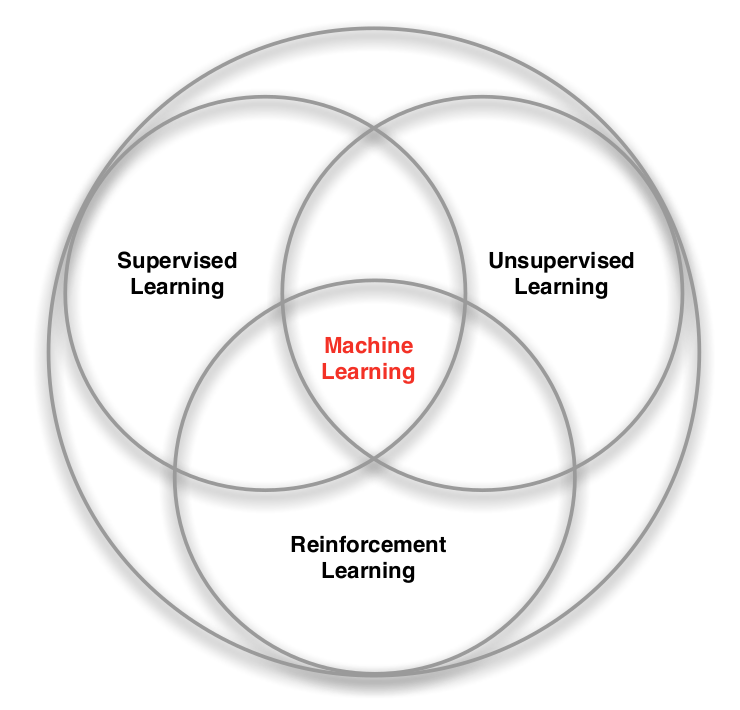
\includegraphics[height=\localheigth]{Figures/RL/RL-machinelearning-chart}
		\label{fig:rl-machinelearning-chart}
	}
	%  	\hspace*{1.5cm} % space between two figures
	\subfigure[]{%
		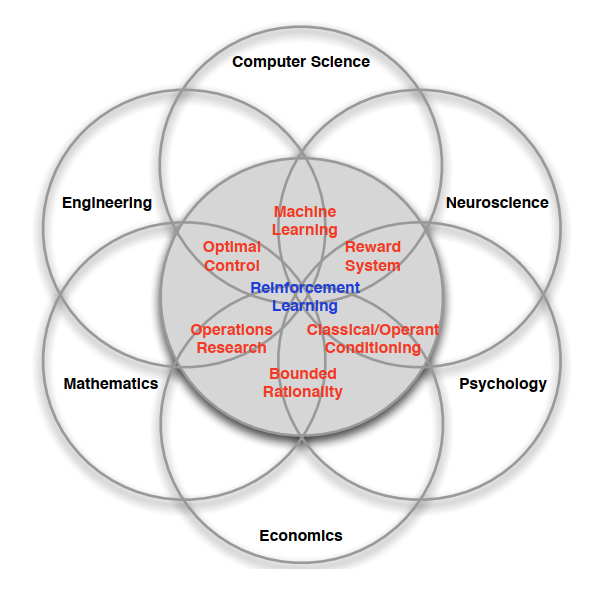
\includegraphics[height=\localheigth]{Figures/RL/RL-chart}
		\label{fig:rl-chart}
	}
	\caption[]{%
	}
	\label{fig:Rl-circle-total}
\end{figure}



\subsection[وجه تمایز 
\ws{rl}
از دیگر الگو‌های 
\ws{ml}
]{چه چیزی 
\ws{rl}
را با دیگر الگوهای 
\ws{ml}
متمایز می‌کند؟
}

\begin{figure}
	\centering
	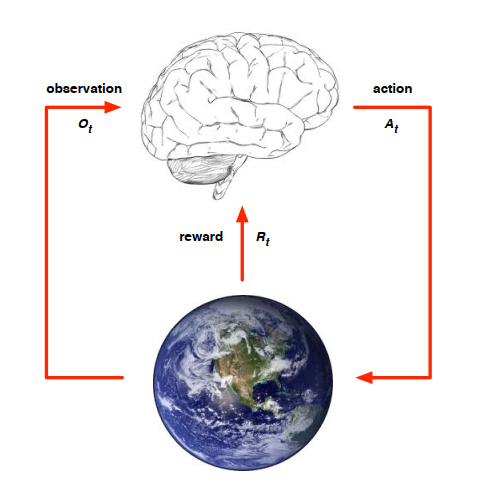
\includegraphics[width=0.7\linewidth]{Figures/RL/Enviroment-brain-as-agent}
	\caption{}
	\label{fig:enviroment-brain-as-agent}
\end{figure}
\begin{figure}
	\centering
	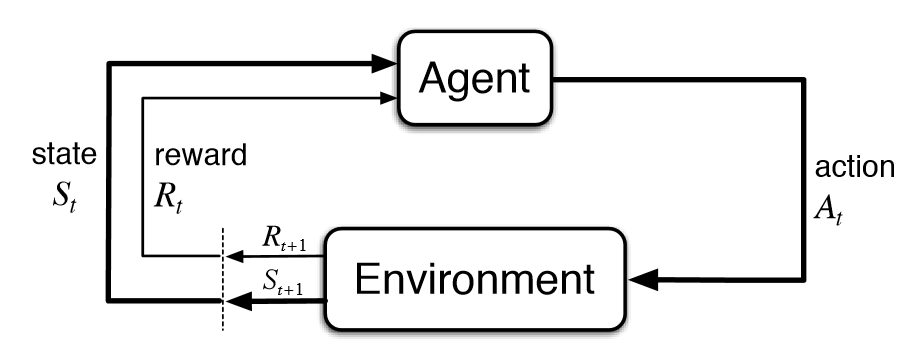
\includegraphics[width=0.7\linewidth]{Figures/RL/Markov-vhain-SARSA}
	\caption{}
	\label{fig:markov-vhain-sarsa}
\end{figure}
\begin{figure}
	\centering
	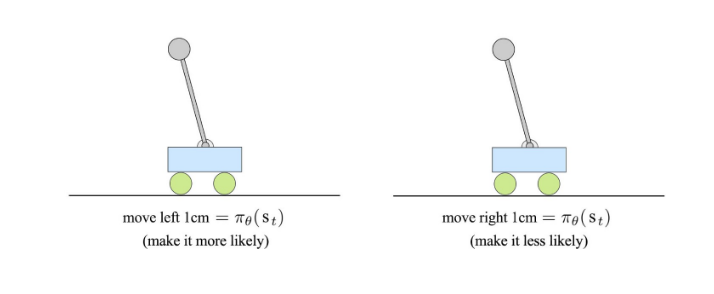
\includegraphics[width=0.7\linewidth]{Figures/RL/RL-cartpole}
	\caption{}
	\label{fig:rl-cartpole}
\end{figure}